% !TeX root = ../main.tex
% Add the above to each chapter to make compiling the PDF easier in some editors.

\chapter{Implementations}\label{chapter:implementations}
This section explains the implementations and how to implement them efficiently. As the shuffle operator-simulation is based on fixed-size tuples, the explanations of the following implementation, are based on fixed-size tuples as well.

\section{Slotted Pages}
TODO: Explain tuple write out process.
\begin{figure}[h]
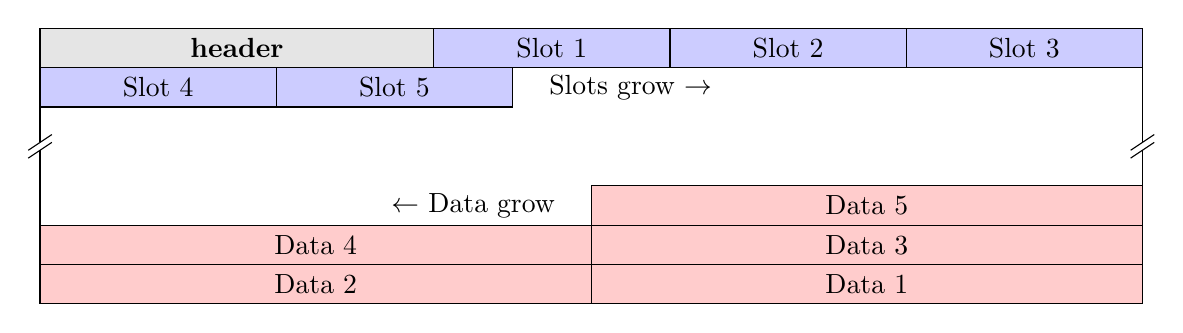
\begin{tikzpicture}
    % Page Outline
    \foreach \x in {0, 14}{
        \draw (\x,0) -- (\x,1.95);
        \draw (\x-0.15,1.85) -- (\x+0.15,2.05);
        \draw (\x,3) -- (\x,2.05);
        \draw (\x-0.15,1.95) -- (\x+0.15,2.15);
    }

    % Header Section
    \fill[gray!20] (0,3) rectangle (5,3.5);
    \node[anchor=center] at (2.5,3.25) {\textbf{header}};
    \draw (0,3) rectangle (5,3.5);

    % Slots Section
    \fill[blue!20] (5,3) rectangle (14,3.5);
    \fill[blue!20] (0,2.5) rectangle (6,3);

    % Slots (Fixed-size entries)
    \foreach \x in {5, 8, 11} {
        \draw (\x,3) rectangle (\x+3,3.5);
        \node[anchor=center] at (\x+1.5,3.25) {Slot \pgfmathparse{(\x-2)/3} \pgfmathprintnumber[precision=0]{\pgfmathresult}};
    }
    \foreach \x in {0, 3} {
        \draw (\x,2.5) rectangle (\x+3,3);
        \node[anchor=center] at (\x+1.5,2.75) {Slot \pgfmathparse{(\x)/3 + 4} \pgfmathprintnumber[precision=0]{\pgfmathresult}};
    }

    \node[anchor=center] at (6+1.5,2.75) {Slots grow $\rightarrow$};


    % Data Section
    \fill[red!20] (7,0) rectangle (14,1.5);
    \fill[red!20] (0,0) rectangle (14,1);

    \foreach \x in {14, 7} {
        \draw (\x,0) rectangle (\x-7,0.5);
        \node[anchor=center] at (\x-3.5,0.25) {Data \pgfmathparse{2-(\x)/7 + 1} \pgfmathprintnumber[precision=0]{\pgfmathresult}};
        \draw (\x,0.5) rectangle (\x-7,1);
        \node[anchor=center] at (\x-3.5,0.75) {Data \pgfmathparse{2-(\x)/7 + 3} \pgfmathprintnumber[precision=0]{\pgfmathresult}};
    }
    \draw (14,1) rectangle (7,1.5);
    \node[anchor=center] at (14-3.5,1.25) {Data \pgfmathparse{2-(14)/7 + 5} \pgfmathprintnumber[precision=0]{\pgfmathresult}};
    \node[anchor=center] at (7-1.5,1.25) {$\leftarrow$ Data grow};

\end{tikzpicture}
\centering
\caption{Slotted Page grow visualization}
\end{figure}

\section{Slotted Page Managers}
As some implementation share the same tuple write-out strategy, we propose the used write-out strategies here and reference them in the following explanations of the concrete implementations.

To further simplify the implementations, we intialize each partition with an empty slotted page. This significantly reduces the complexity of the page manager implementations.

\subsection{Lock-based Page Manager}
For each partition, we use a single lock and a vector for storing the slotted pages.
\begin{algorithm}[h]
\caption{Lock-based Page Manager insert\_tuple Algorithm}\label{Lock-based-page-manager-insert-tuple}
\SetKwInOut{Input}{input}\SetKwInOut{Output}{output}
\Input{\texttt{tuple}: The tuple to be inserted, \texttt{partition}: The target partition index}
\Output{Tuple inserted into the appropriate slotted page of the specified partition.}

\SetKwFunction{Insert}{ insert\_tuple}

\textbf{function}\Insert{tuple, partition}{

    Acquire lock on \texttt{partition\_locks[partition]}\;
    \eIf{pages[partition].back().add\_tuple(tuple)}{
        // Tuple added successfully\;
    }{
        add\_page(partition)\;
        pages[partition].back().add\_tuple(tuple)\;
    }
    Release lock\;
}
\end{algorithm}
As can be seen in Algorithm \ref{Lock-based-page-manager-insert-tuple}, the lock-based insertion process is straightforward.
The insertion on a given slotted page, can only fail if the page is full.
This can easily be checked by reading the tuple count in the metadata section of the slotted page.
If the current page is full, we just allocate and append a new slotted page to the page vector of this partition.

\subsubsection*{Tuple insertion in batches}
Similarly, we can further optimize the write-out by using tuple-batches.
\begin{algorithm}[h]
\caption{Lock-based Page Manager insert\_tuple\_batch Algorithm}\label{Lock-based-page-manager-insert-tuple-batch}
\SetKwInOut{Input}{input}\SetKwInOut{Output}{output}
\Input{\texttt{tuples}: The tuple-batch to be inserted\\ \texttt{partition}: The target partition index}
\Output{Tuples inserted into one or more slotted pages of the specified partition.}

\SetKwFunction{Insert}{ insert\_tuple\_batch}

\textbf{function}\Insert{tuples, partition}{

    Acquire lock on \texttt{partition\_locks[partition]}\;
    \For{tuple : tuples}{
    \eIf{pages[partition].back().add\_tuple(tuple)}{
        // Tuple added successfully\;
    }{
        add\_page(partition)\;
        pages[partition].back().add\_tuple(tuple)\;
    }}
    Release lock\;
}
\end{algorithm}
In Algorithm \ref{Lock-based-page-manager-insert-tuple-batch}, we reuse the tuple insertion logic from Algorithm \ref{Lock-based-page-manager-insert-tuple} but acquire the partition lock only once for the entire insertion process.
Since acquiring and releasing the lock is expensive, this optimization significantly improves performance in multi-threaded scenarios.

\subsection{Lock-free Page Manager}
As holding a lock of a partition denies a second thread to also write out tuples, we propose a lock-free implementation.
In comparision to the lock-based variant, we now have to store our slotted pages in a pointer-stable data structure.
This is necessary to ensure threads can work simultanious, while a thread adds a new slotted page.
Furthermore, we have to edit the slotted page metadata using compare-and-exchange operations to avoid losing writes from other threads.



\begin{algorithm}[h]
\caption{Lock-free Slotted Page increment\_and\_fetch\_opt\_write\_info Algorithm}\label{Lock-free-page-increment}
\SetKwFunction{Increment}{ increment\_and\_fetch\_opt\_write\_info}
\textbf{function}\Increment{}{

current\_tuple\_count = header->tuple\_count.load();

\While{!header->tuple\_count.compare\_exchange\_strong(current\_tuple\_count, current\_tuple\_count + 1)} {
    \If {current\_tuple\_count >= get\_max\_tuples(page\_size)} {
        return std::nullopt\;
    }
}

return \{page\_data.get(), page\_size, current\_tuple\_count\}\;
}\end{algorithm}
In order to gather the information, where we can write a tuple, we increment the tuple count using compare-and-exchange.
This index then acts as our location, where our tuple is placed on the page.
In Algorithm \ref{Lock-free-page-increment}, we also add an condition to stop attempting to further increase the count of tuples on the page, if the maximum is reached.
This ensures that threads move to the next allocated page. Given the index, where the tuple is placed, we also append a pointer of the start of the page and the page size.
This ensures we can write the page without requiring any further information.

\begin{algorithm}[h]
\SetKwFunction{Insert}{ insert\_tuple}
\caption{Lock-free Page Manager insert\_tuple Algorithm}\label{Lock-free-page-manager-insert-tuple}
\SetKwInOut{Input}{input}\SetKwInOut{Output}{output}
\Input{\texttt{tuple}: The tuple to be inserted, \texttt{partition}: The target partition index}
\Output{Tuple inserted into the appropriate slotted page of the specified partition.}
\textbf{function}\Insert{tuple, partition}{

    wi = current\_page[partition].load()->increment\_and\_fetch\_opt\_write\_info()\;
    \While{wi == std::nullopt}{
        wi = current\_page[partition].load()->increment\_and\_fetch\_opt\_write\_info()\;
    }
    \If{wi.tuple\_index == LockFreeSlottedPage::get\_max\_tuples() - 1}{
        add\_page(partition)\;
    }
    LockFreeSlottedPage::add\_tuple\_using\_index(wi, tuple)\;
}
\end{algorithm}
Using the Algorithm \ref{Lock-free-page-increment}, we retrieve the information to write the tuple in Algorithm \ref{Lock-free-page-manager-insert-tuple}.
We read from an atomically-stored pointer to our current page, until we are assigned an index on a slotted page.
If we are writing the last tuple on the page, we add a new page to this partition.
This is necessary to create a unqiue condition, when a new page has to be allocated.
With that write information at hand, we can write the tuple onto the slotted page.
\subsection{Histogram-based Page Managers}
\subsubsection{Radix Page Manager}
\subsubsection{Ad-hoc Radix ("Hybrid") Page Manager}

\subsection{Thread-Local Pages and Merge-based Page Manager}

\subsection{Implementation-independent Optimizations}
\subsubsection{Padded atomics and locks}
\subsubsection{Minimal page-locking}
\subsubsection{Two-step buffered slotted page write out}

\section{On-Demand Partitioning}
On-demand Partitioning is the simplest algorithm to implement the shuffle operator.
\subsection{Overview}
As soon as this implementation receives a batch of tuples, it processes each tuple individually. First, the hash-function is applied onto the tuple to gather information in which partition this tuple belongs. With this information, we only need to write out the tuple into the corresponding partition. The partition is now locked, and we check, if there is enough space left on the newest slotted page of this partition.

%If this is the case, we first check if this page can fit at least another tuple. This is necessary to create a unique condition, when a new page has to be allocated. If the current tuple will be the last tuple of this page, we must also create a new slotted page for this partition.

%Otherwise,
\section{Software Managed Buffers-based Partitioning}
\subsection{Overview}
\subsection{Lock-based Implementations}
\subsection{Lock-free Implementations}

\section{Histogram-based Partitioning}
\subsection{Overview}
\subsection{Radix Partitioning}
\subsection{Ad-hoc Radix ("Hybrid") Partitioning}

\section{Thread-Local Pages and Merge-based Partitioning}
\subsection{Overview}

\section{Collaborative Morsel Processing}
\subsection{Overview}
\subsection{Collaborative Morsel Processing using Software Managed Buffers}
\subsection{Collaborative Morsel Processing using Processing Units}

\section{Complexity Analysis}
\subsection{Time Complexity}
%$\Theta(n)$
\subsubsection{Tuple Access Count}
\subsection{Space Complexity}
%$\Theta(n)$
\subsubsection{Memory Consumption}
